\section{Software}

El desarrollo del software del robot militar se realizó siguiendo el paradigma de Programación Orientada a Objetos (POO), permitiendo una estructura modular y escalable. Esta arquitectura facilita la separación clara de responsabilidades, el mantenimiento del código y la posibilidad de extender funcionalidades sin afectar el comportamiento general del sistema.

El sistema está dividido en tres módulos principales: control de misión, navegación autónoma y seguimiento de objetivos. Cada uno de estos módulos interactúa a través de interfaces bien definidas, lo que permite la sustitución o mejora de componentes sin necesidad de modificar el resto del sistema.

\begin{itemize}
    \item \textbf{Control de misión:} Administra el estado general del robot y coordina los distintos subsistemas según el tipo de misión. Incluye lógica para transiciones entre estados como patrullaje, búsqueda de objetivos, eliminación y navegación hacia puntos estratégicos. También gestiona el tiempo de ejecución y las condiciones de activación de cada misión.

    \item \textbf{Seguimiento de objetivos:} Utiliza técnicas de visión computacional para analizar imágenes recibidas en tiempo real y detectar objetivos. Emplea controladores PID para alinear la torreta del robot con el objetivo detectado y evalúa condiciones de disparo según el nivel de precisión alcanzado.

    \item \textbf{Navegación autónoma:} Se basa en mapas de ocupación del entorno y algoritmos de planificación de trayectorias para determinar rutas seguras hacia los puntos de interés. Este módulo considera tanto la posición como la orientación del robot, y ajusta los comandos de movimiento para alcanzar los objetivos de forma precisa y eficiente.

    \item \textbf{Interfaces modulares:} El sistema fue diseñado para funcionar tanto en un entorno simulado como en uno real. Para ello, se implementaron drivers abstractos que permiten controlar el robot mediante simuladores (como gamepads virtuales) o hardware real sin alterar la lógica del sistema principal. De igual manera, la comunicación entre módulos se realiza mediante un sistema de colas de mensajes, que asegura una interacción desacoplada y eficiente entre procesos.

\end{itemize}

Gracias a esta estructura modular y orientada a objetos, el software no solo puede adaptarse a distintos escenarios operativos, sino que también facilita futuras mejoras, pruebas automatizadas y escalabilidad hacia sistemas más complejos o entornos reales de combate.

\subsection{Máquina de Estados Finitos}

El comportamiento general del robot se organiza como una máquina de estados finitos (FSM, por sus siglas en inglés), lo que permite una lógica de control clara, robusta y fácilmente extensible. Cada estado representa una configuración operativa particular del robot, y las transiciones entre ellos se determinan en función de eventos y condiciones específicas del entorno o de la misión.

\subsubsection{Estados Principales}

\begin{itemize}
    \item \textbf{STARTING:} Estado inicial del sistema. Evalúa el tipo de misión configurada y decide si comenzar en modo \texttt{SENTINEL} o \texttt{NAVIGATING}.

    \item \textbf{SENTINEL:} Modo de vigilancia estática en el que el robot escanea el entorno en busca de objetivos utilizando visión computacional. Si se detecta un objetivo, se transiciona al estado \texttt{TRACKING}.

    \item \textbf{TRACKING:} El robot ajusta la orientación de su torreta para seguir un objetivo en movimiento. Si logra un seguimiento preciso, transiciona al estado \texttt{TRACK\_N\_KILL}. Si pierde el objetivo, regresa a \texttt{SENTINEL} o \texttt{NAVIGATING}, dependiendo del estado anterior interrumpido.

    \item \textbf{TRACK\_N\_KILL:} Estado en el cual el robot ha fijado un blanco con alta precisión y activa su mecanismo de ataque. Si se pierde la fijación, vuelve a \texttt{TRACKING}.

    \item \textbf{NAVIGATING:} Estado de navegación autónoma hacia puntos estratégicos definidos en la misión. Si se detecta un objetivo durante la marcha, el sistema cambia a \texttt{TRACKING}. Al alcanzar un objetivo con tipo de misión de vigilancia, cambia a \texttt{SENTINEL}.

    \item \textbf{IDLE / PATROLLING / MAPPING:} Estados secundarios que permiten al robot detenerse, patrullar o explorar el entorno. Aunque no fueron parte del flujo principal en el prototipo básico, están contemplados para futuras funcionalidades.

    \item \textbf{DEBUG / ERROR:} Estados especiales para depuración o manejo de fallas críticas en tiempo de ejecución.
\end{itemize}

\subsection*{Transiciones}

Las transiciones entre estados se determinan mediante condiciones lógicas evaluadas en tiempo real:

\begin{itemize}
    \item \textbf{STARTING $\rightarrow$ SENTINEL/NAVIGATING:} Según si la misión es de vigilancia estática o de desplazamiento.
    \item \textbf{SENTINEL $\rightarrow$ TRACKING:} Activada cuando el sistema de visión detecta un objetivo.
    \item \textbf{TRACKING $\rightarrow$ TRACK\_N\_KILL:} Cuando el objetivo está centrado y estable.
    \item \textbf{TRACKING $\rightarrow$ SENTINEL/NAVIGATING:} Si se pierde el objetivo, se regresa al estado anterior.
    \item \textbf{TRACK\_N\_KILL $\rightarrow$ TRACKING:} Si se pierde la fijación sobre el objetivo.
    \item \textbf{NAVIGATING $\rightarrow$ TRACKING:} Si se detecta un objetivo durante el trayecto.
    \item \textbf{NAVIGATING $\rightarrow$ SENTINEL:} Cuando se alcanza el destino y el tipo de misión lo requiere.
\end{itemize}

Este enfoque basado en FSM proporciona una estructura robusta y predecible para la toma de decisiones del robot, facilitando además su validación mediante pruebas controladas y su extensión hacia escenarios más complejos.

\begin{figure}[htbp]
\centering
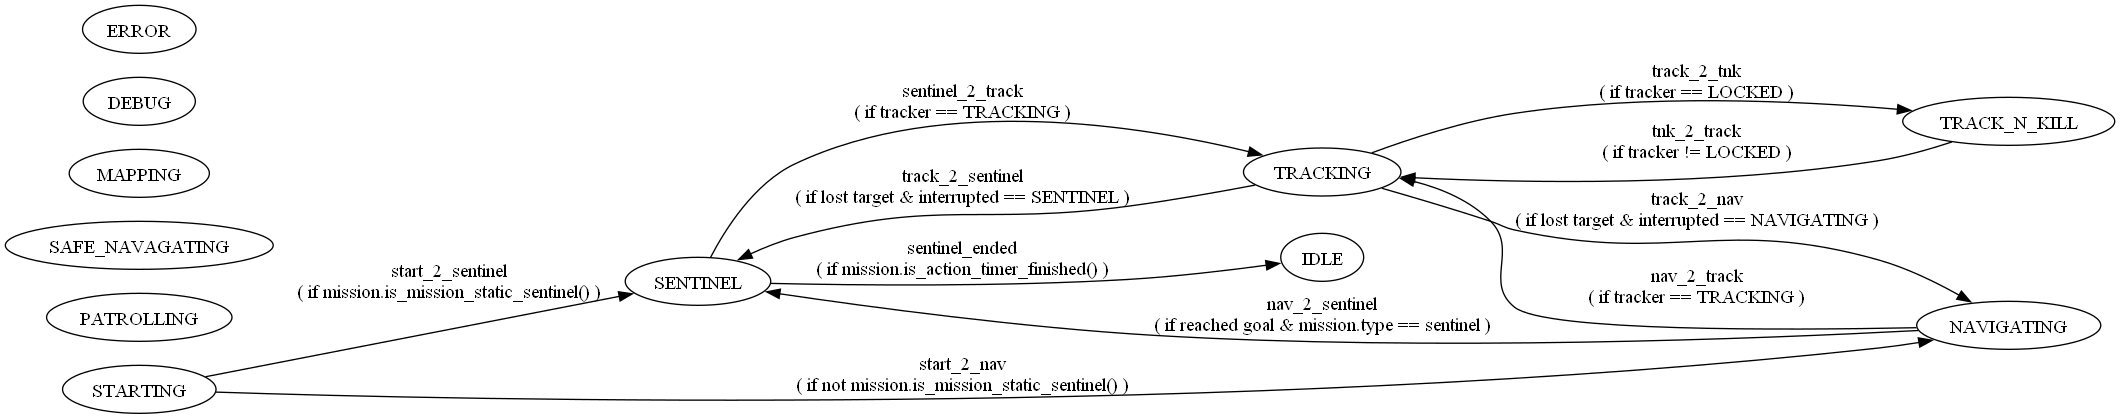
\includegraphics[width=.99\textwidth]{Figures/maquina_de_estados.png}
\label{fig:Maquina_de_estado}
\caption{Máquina de estados finitos del prototipo}
\end{figure}

\subsection{Análisis de Implementación}

A continuación, se presenta un análisis detallado de la implementación del sistema, organizado en subsecciones que corresponden a los componentes clave del software. Este análisis se centra en el funcionamiento y el rol de cada componente dentro del sistema global, destacando los aspectos teóricos y las decisiones de diseño que sustentan su desarrollo. Cuando es relevante, se incluyen fragmentos de código para ilustrar conceptos específicos.

\subsubsection{Control Central y Coordinación de Módulos}

El componente central de control actúa como el núcleo del sistema robótico, encargado de coordinar las interacciones entre los módulos de seguimiento de objetivos y navegación autónoma, además de gestionar las transiciones de estado según la máquina de estados finitos descrita. Su rol principal es asegurar que el robot opere de manera coherente, alternando entre diferentes comportamientos según las condiciones de la misión y los eventos del entorno.

Desde un punto de vista teórico, este componente implementa un patrón de diseño de \textit{mediador}, donde un elemento central coordina las interacciones entre múltiples subsistemas sin que estos se comuniquen directamente entre sí. Esto reduce el acoplamiento y mejora la modularidad, ya que los módulos solo interactúan con el controlador central a través de interfaces bien definidas. Además, la capacidad de inicializar diferentes tipos de controladores para hardware virtual o real refleja el principio de \textit{inversión de dependencias}, permitiendo que el sistema sea independiente de la implementación específica del hardware.

El bucle principal del sistema actualiza continuamente la posición y orientación del robot mediante mensajes recibidos de un sistema de colas de mensajería. Este enfoque de procesamiento basado en eventos es típico en sistemas reactivos, donde el robot debe responder en tiempo real a cambios en el entorno o a nuevas detecciones de objetivos. Un aspecto crítico del diseño es la gestión de interrupciones, como cuando se detecta un objetivo durante la navegación. El sistema guarda el estado anterior para permitir la reanudación de la tarea original una vez que se pierde el objetivo, lo que demuestra un manejo robusto de prioridades en un entorno dinámico.

\subsubsection{Seguimiento de Objetivos y Control de Torreta}

El módulo de seguimiento de objetivos es responsable de detectar y seguir objetivos mediante visión computacional, así como de controlar la torreta del robot para alinearla con el objetivo detectado. Su rol es crucial en las fases de vigilancia y ataque, permitiendo al robot identificar amenazas y actuar en consecuencia.


Este módulo utiliza un controlador PI (Proporcional-Integral), que combina términos proporcional e integral para minimizar el error entre la posición deseada y la actual de la torreta. Se optó por no incluir el término derivativo debido a que puede amplificar el ruido presente en las mediciones de la cámara y causar movimientos erráticos de la torreta. En la implementación, se observa cómo se limitan los valores integrales y de salida para evitar comportamientos inestables, como oscilaciones excesivas. A continuación, se muestra un fragmento de código que ilustra este control PI:

\begin{lstlisting}[language=Python, caption=Control PI para seguimiento de objetivos, label=lst:control_pi]
# Detectar objetivo en la imagen
objetivo = detectar_objetivo(imagen_camara)

# Calcular error de posicion respecto al centro
error_actual = calcular_error(objetivo, centro_pantalla)

# Aplicar control PI (sin termino derivativo)
error_proporcional = error_actual
error_integral += error_actual
salida_pi = Kp * error_proporcional + Ki * error_integral

# Limitar salida para evitar oscilaciones
salida_limitada = limitar_salida(salida_pi)

# Ajustar orientacion de la torreta
torreta.mover(salida_limitada)

# Si el objetivo esta centrado, activar disparo
if objetivo_centrado(error_actual):
    sistema_disparo.activar()
\end{lstlisting}
El módulo procesa datos de video recibidos a través de un sistema de mensajería, filtrando objetivos según una etiqueta específica y calculando el centro del cuadro delimitador del objetivo con mayor confianza. Luego, determina si el objetivo está dentro de un margen de seguridad para decidir si está en modo de bloqueo (listo para disparar) o de seguimiento activo. Este enfoque de umbral binario simplifica la decisión de disparo, aunque podría mejorarse con técnicas más avanzadas como filtros de Kalman para suavizar las trayectorias de seguimiento.

Además, cuando no hay objetivos detectados, el módulo implementa un comportamiento de búsqueda, moviendo la torreta en un patrón de barrido definido por ángulos máximos y mínimos. Este comportamiento refleja un enfoque de exploración sistemática, común en sistemas de vigilancia autónoma.

\subsubsection{Navegación Autónoma y Planificación de Rutas}

El módulo de navegación autónoma gestiona el desplazamiento del robot hacia puntos de interés definidos en una misión. Su rol es determinar rutas seguras y eficientes utilizando mapas de ocupación del entorno y algoritmos de planificación de trayectorias, asegurando que el robot alcance sus objetivos mientras evita obstáculos.

Desde una perspectiva teórica, la navegación autónoma integra localización, mapeo y planificación de rutas. Este módulo calcula rutas óptimas mediante el algoritmo A*, como se discutió en la sección teórica previa. Carga un mapa de ocupación y genera una ruta hacia el objetivo, almacenando los puntos intermedios (waypoints) para su seguimiento. El control de movimiento ajusta la velocidad lineal y angular del robot en función de la distancia y el ángulo hacia el objetivo, utilizando un enfoque proporcional simple para evitar sobrepasar el destino, como se muestra en el siguiente fragmento:

\begin{lstlisting}[language=Python, caption=Control proporcional para navegación, label=lst:control_proporcional]
# Calcular distancia al objetivo
distancia_al_objetivo = calcular_distancia(posicion_actual, objetivo)

# Control proporcional de velocidad
velocidad_adelante = distancia_al_objetivo * ganancia_velocidad
velocidad_adelante = limitar_velocidad(velocidad_adelante)

# Calcular error angular y ajustar giro
error_angular = calcular_error_orientacion(objetivo)
velocidad_giro = error_angular * ganancia_giro
velocidad_giro = limitar_giro(velocidad_giro)

# Mover el robot
robot.mover(velocidad_adelante, velocidad_giro)
\end{lstlisting}

Este método podría beneficiarse de controladores más sofisticados como PID o MPC (Model Predictive Control) para manejar dinámicas más complejas o terrenos irregulares. Un aspecto notable es el registro de la trayectoria del robot, que se guarda para análisis posterior y depuración, un aspecto crucial en el desarrollo de sistemas autónomos.

\subsubsection{Comunicación y Mensajería entre Módulos}

El sistema de comunicación basado en colas de mensajes es fundamental para la arquitectura desacoplada del software, permitiendo que los módulos intercambien datos como imágenes procesadas o información de posición sin una conexión directa. Su rol es asegurar una interacción eficiente y asíncrona entre los componentes del sistema.

Teóricamente, este sistema implementa el patrón de diseño \textit{publish-subscribe} combinado con colas de trabajo, lo que asegura que los mensajes sean persistentes y procesados de manera ordenada. Permite a los módulos acceder a los datos más recientes o limpiar la cola para evitar acumulación de mensajes obsoletos, lo que es crítico en aplicaciones en tiempo real donde la latencia debe minimizarse. Este enfoque de comunicación asíncrona es ideal para sistemas distribuidos, ya que permite que los componentes operen de manera independiente y a diferentes velocidades de procesamiento. Sin embargo, introduce desafíos como la gestión de errores en la decodificación de mensajes y la posible pérdida de datos si no se implementan mecanismos de confirmación adecuados.

\subsubsection{Configuración y Modularidad del Sistema}

Un tema recurrente en la implementación es el uso de archivos de configuración para parametrizar el comportamiento del sistema. Esto se observa en la inicialización de todos los módulos principales, donde parámetros como ganancias de control, márgenes de seguridad y configuraciones de hardware se cargan dinámicamente. Desde un punto de vista teórico, este enfoque sigue el principio de \textit{configuración sobre convención}, permitiendo ajustes sin modificar la lógica interna, lo que es esencial para pruebas y adaptaciones a diferentes entornos o hardware.

Además, la modularidad se refuerza mediante el uso de controladores virtuales que abstraen la interacción con el hardware. Esto refleja el patrón de diseño \textit{adaptador}, facilitando la transición entre simulación y operación real, un aspecto clave en el desarrollo de sistemas robóticos donde las pruebas en hardware físico pueden ser costosas o peligrosas.

\subsection{Conclusiones del Análisis de Implementación}

El análisis de la implementación revela un diseño de software bien estructurado, basado en principios de modularidad, desacoplamiento y configurabilidad. La implementación de una máquina de estados finitos proporciona un marco robusto para la toma de decisiones, mientras que los módulos de seguimiento y navegación utilizan técnicas de control clásicas y modernas para cumplir con los objetivos de la misión. El sistema de comunicación asegura una interacción eficiente entre componentes, aunque podría beneficiarse de mecanismos adicionales de manejo de errores y sincronización.

En términos teóricos, el software refleja una combinación de enfoques reactivos y deliberativos: reactivos en la respuesta inmediata a detecciones de objetivos, y deliberativos en la planificación de rutas y gestión de misiones. Esta dualidad es típica en robótica autónoma, donde se requiere un equilibrio entre rapidez de respuesta y planificación a largo plazo. Futuras mejoras podrían incluir la integración de algoritmos de aprendizaje automático para la adaptación dinámica de parámetros de control y la implementación de técnicas de fusión de sensores para mejorar la robustez en entornos complejos.